\DiaryEntry{Linear Programs}{2022-09-27}{Optimization}

\subsection{Introduction}

This is based on \cite{Sierksma2015} which uses the model "Dovetail",

\begin{align*}
  \max \; & 3x_1 + 2x_2 \\
       & x_1 + x_2 \leq 9 \\
       & 3x_1 + x_2 \leq 18 \\
       & x_1 \leq 7 \\
       & x_2 \leq 6 \\
       & x_1, x_2 \geq 0
\end{align*}

The Figure below shows the feasible region $\Fc$ of the model together with the inequalities and the vertices.

\begin{figure}[H]
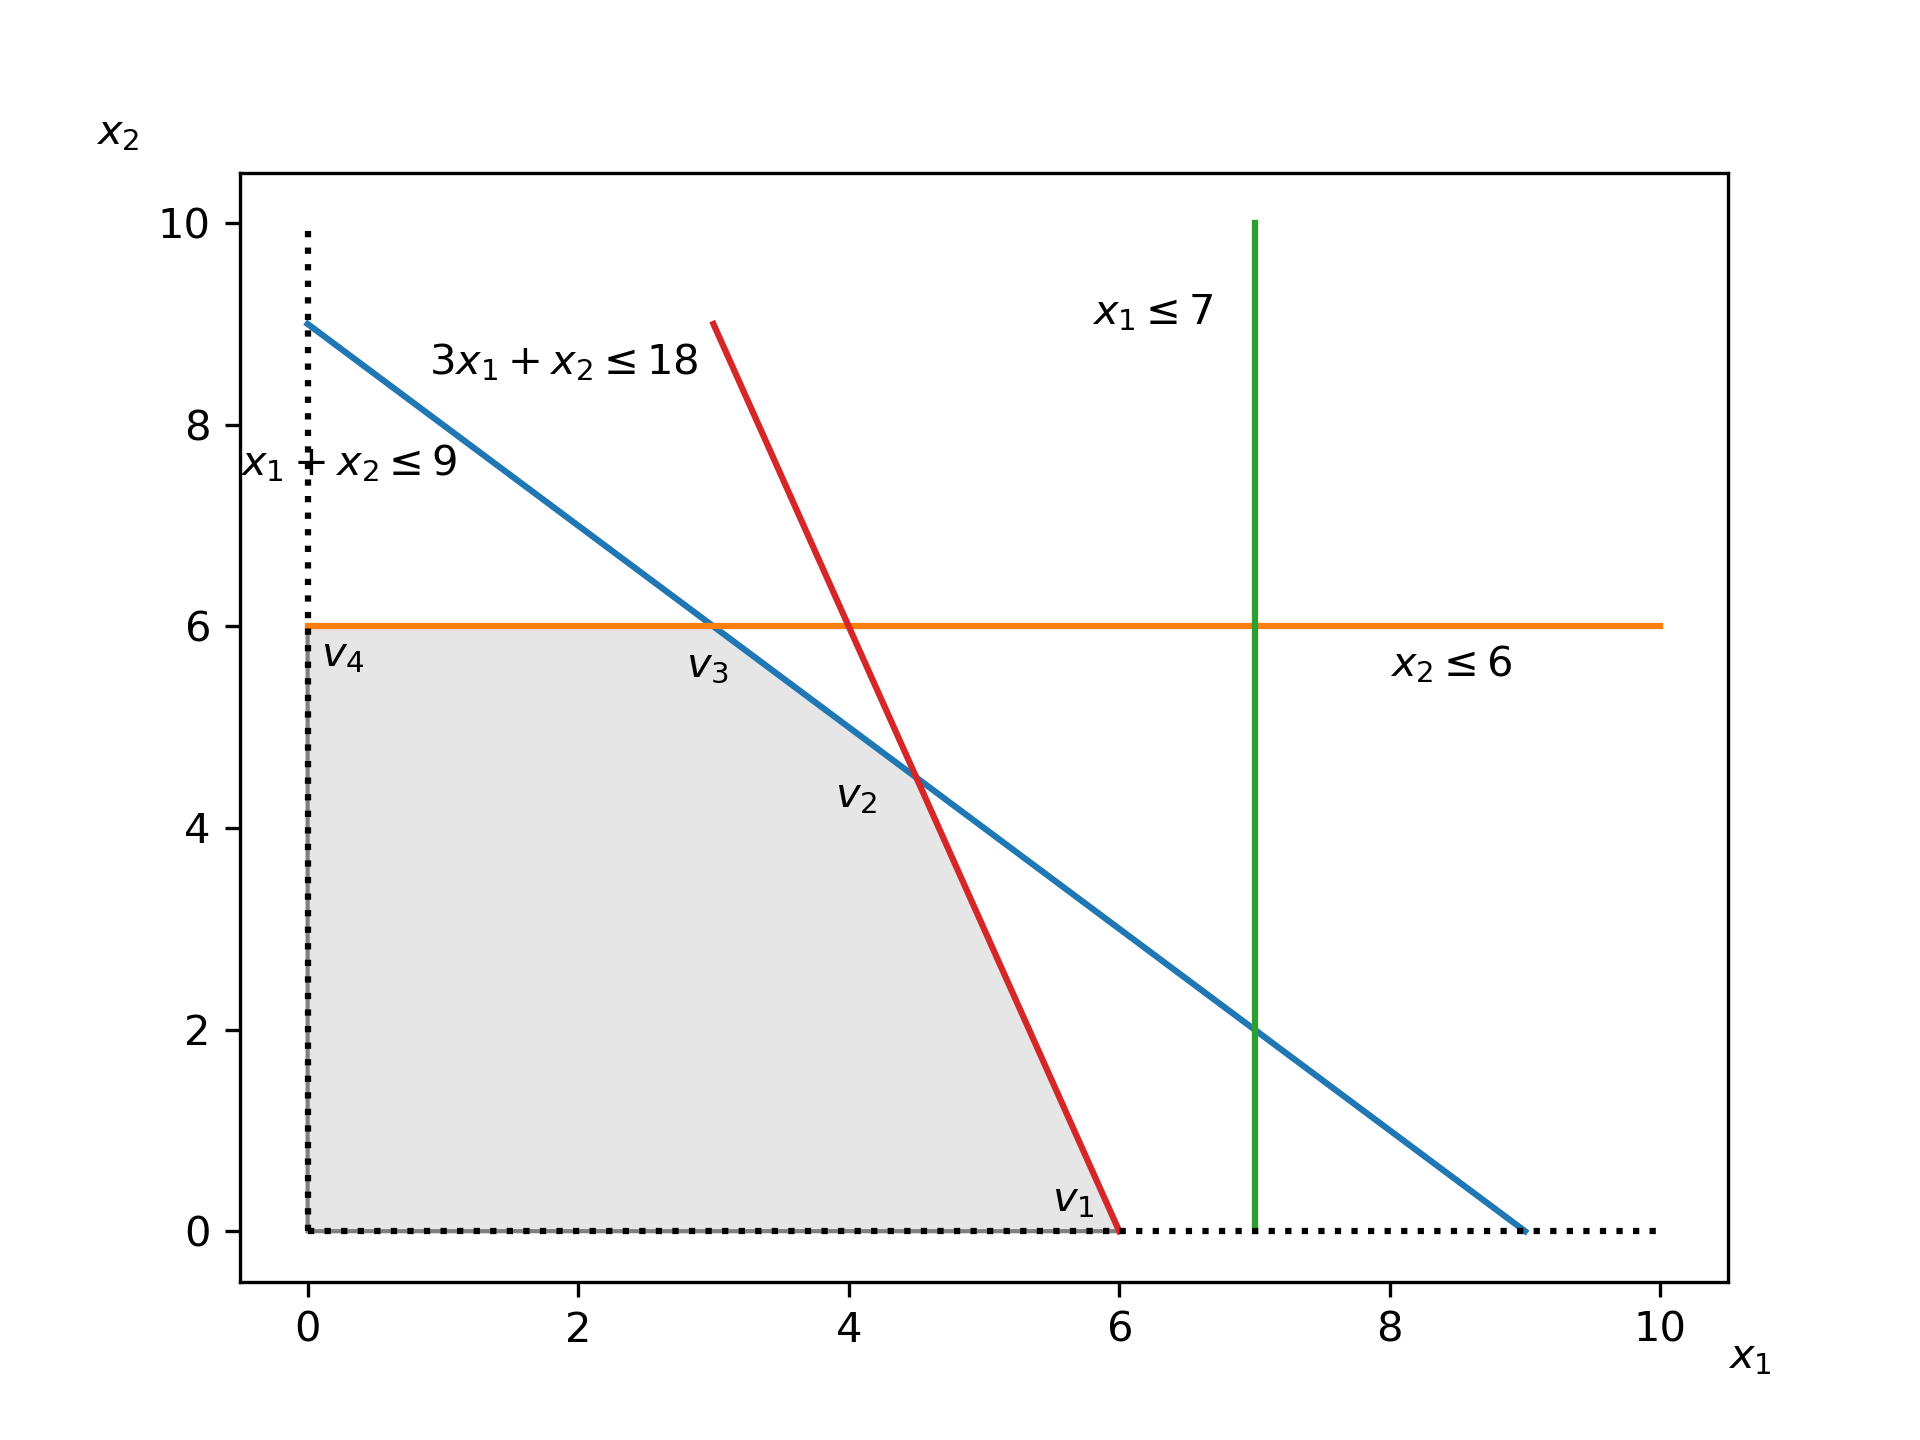
\includegraphics[scale = 0.7]{images/2022-09-27_lin_prog_1_01.png}
\end{figure}

We can rewrite the constraints in matrix-vector form. We split the constraints into \emph{non-negativity} constraints ($x_1, x_2 \geq 0$) and \emph{technology constraints} (all other constraints). Define $\xbf = [x_1, x_2]^T$ and then we get

\bee
\max \cbf^T \xbf, \quad \text{subject to} \; \Abf \xbf \leq \bbf, \xbf \geq \zerobf
\eee

with $\cbf = [3, 2]^T, \bbf = [9, 18, 7, 6]^T$ and the \emph{technology matrix}

\bee
\Abf = \begin{pmatrix} 1 & 1 \\ 3 & 1 \\ 1 & 0 \\ 0 & 1 \end{pmatrix} 
\eee

\paragraph{Slack Variables.} We can rewrite inequality constraints as equality constraints by introducing an additional variable called a \emph{slack variable}. As an example, the constraints $x_1 + x_2 \leq 9, x_1, x_2 \geq 0$ become

\bee
x_1 + x_2 + x_3 = 9, \quad x_1, x_2, x_3 \geq 0
\eee

The slack variable variable $x_3$ measures how far away we are from the equality constraint $x_1 + x_2 = 9$. If $x_3 > 0$, then we do not fully utilize the constraint. We can convert all inequality constraints into equality by introducing additional slack variables. We collect these into a vector $\xbf_s$ and then our linear program becomes

\bee
\max \cbf^T \xbf, \quad \text{subject to} \; [ \Abf \Ibf ] [ \xbf^T \xbf_s^T]^T = \bbf, \xbf \geq \zerobf, \xbf_s \geq \zerobf
\eee

In our Dovetail example, we have

\begin{align}
  &\max [3, 2]^T \xbf \\
  &\text{subject to} \; \begin{pmatrix} 1 & 1 & 1 & 0 & 0 & 0 \\ 3 & 1 & 0 & 1 & 0 & 0 \\ 1 & 0 & 0 & 0 & 1 & 0 \\ 0 & 1 & 0 & 0 & 0 & 1 \end{pmatrix} [x_1, x_2, x_3, x_4, x_5, x_6]^T = [9, 18, 7, 6]^T \\
  & x_1, \ldots , x_7 \geq 0
\end{align*}


\subsection{Feasible Region}

\paragraph{Hyperplanes and Halfspaces.} Let $n \geq 1$. A hyperplane $H$ in $\mR^n$ is an $n-1$-dimensional set of points satisfying a linear equation of the form

\bee
\abf^T \xbf = b
\eee

Note that this can be rewritten as

\bee
\abf^T (\xbf - \dbf) = \zerobf
\eee

where $\abf^T \dbf = b$. From this definition we can see that the hyperplane goes through the point $\dbf$ and is orthogonal to the vector $\abf$.

The hyperplane separates $\mR^n$ into two halfspaces, one ``below'' and one ``above'' the hyperplane,

\begin{align*}
  H^+ &= \{ \xbf \in \mR^n | \abf^T \xbf \leq b\} \\
  H^- &= \{ \xbf \in \mR^n | \abf^T \xbf \geq b\}
\end{align*}

The definition is such that the intersection of the two hyperplanes gives the hyperplane, $H^+ \cap H^- = H$.

In our Dovetail example, the first constraint $x_1 + x_2 \leq 9$ yields the hyperplane $H_1: x_1 + x_2 = 9$ and the two halfspaces $H_1^+ =  \{ \xbf \in \mR^n | x_1 + x_2 \leq 9 \}$ and $H_1^- =  \{ \xbf \in \mR^n | x_1 + x_2 \geq 9 \}$.

\paragraph{Vertices and Extreme Directions.} There are three equivalent definitions to define a vertex $\xbf_0$ of a feasible region $\Fc$,

\begin{itemize}
  \item $\xbf_0$ is a vertex of $\Fc$, if there are $n$ independent hyperplanes in $\{H_1, H_2, \cdots\}$ that intersect at $\xbf_0$.

  \item $\xbf_0$ is a vertex of $\Fc$, if there is \emph{some} hyperplane $H$ (not necessarily in $\{H_1, H_2, \cdots\}$) with a halfspace $H^+$ such that $F \subseteq H^+$ and $F \cap H = \{ \xbf_0 \}$.

  \item $\xbf_0$ is a vertex of $\Fc$, if there are no two distinct points $\xbf', \xbf'' \in \Fc$, such that $\xbf_0 = \lambda \xbf' + (1-\lambda) \xbf''$ with $\lambda \in (0,1)$.

\end{itemize}

In the first definition, the crucial point is that we need an intersection of $n$ hyperplanes to obtain a vertex \emph{point}. The second one is a bit unusual; a suitable hyperplane is shown in the Figure below: The yellow line is a hyperplane $H$ such that $F \subseteq H^+$ and $\vbf_3$ lies at the interesection of $\Fc$ and $H$ and is therefore a vertex of $\Fc$. Finally, definition three ensures that a vertex lies at ``the corner'' of the feasible region; e.g. we cannot express $\vbf_3$ as convex combintion of two points $\xbf', \xbf'' \in \Fc$ with neither of them being $\vbf_3$.x


\begin{figure}[H]
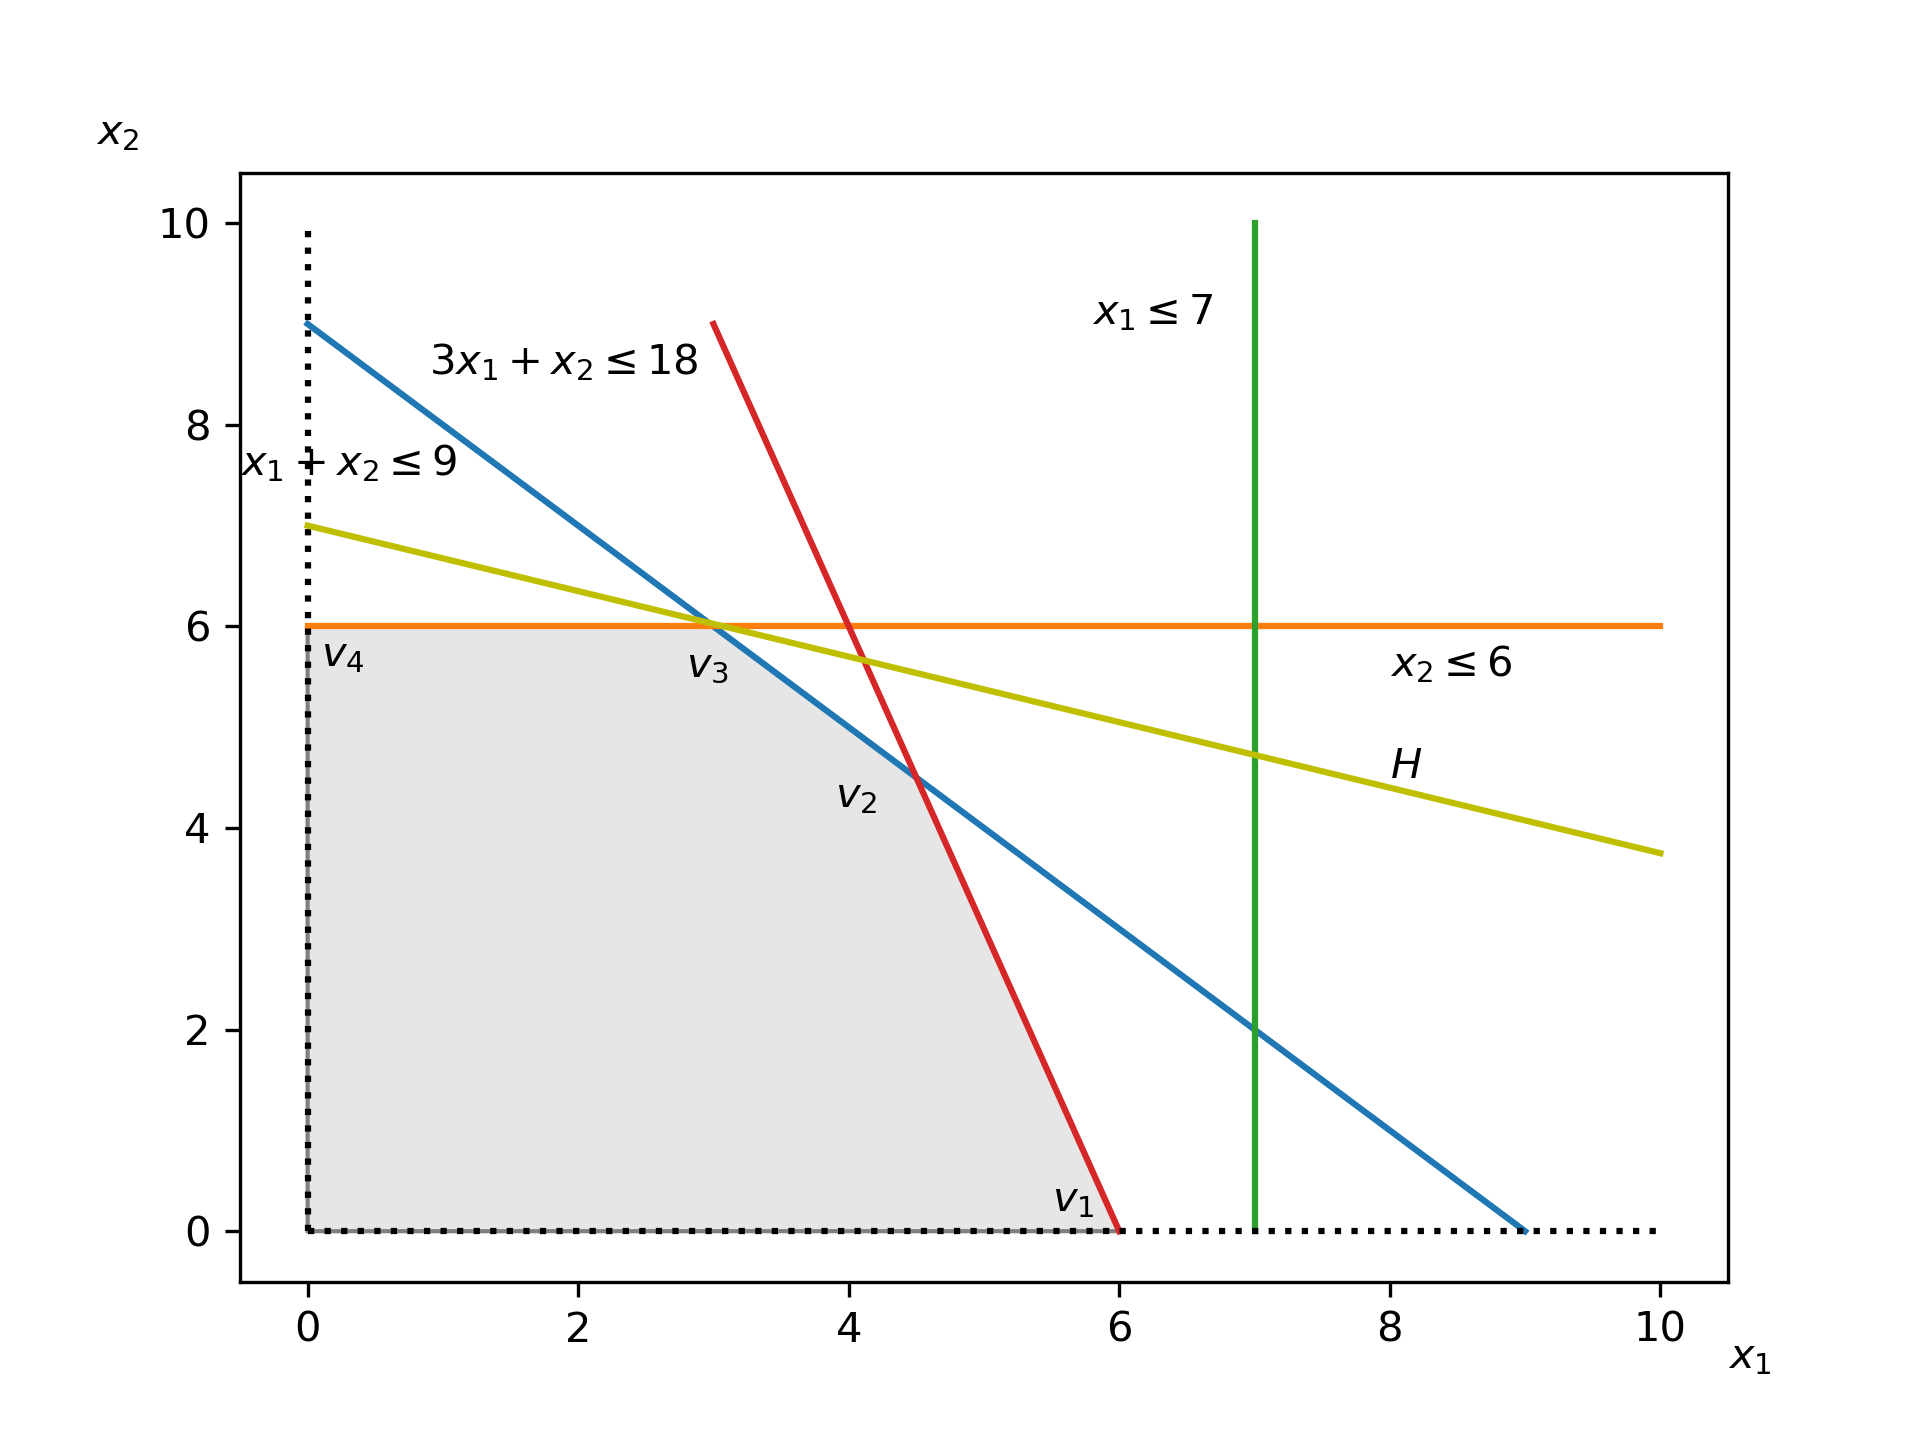
\includegraphics[scale = 0.7]{images/2022-09-27_lin_prog_1_02.png}
\end{figure}

In the case of the Dovetail model, the vertices describe the full feasible region in the sense that the feasible region is the convex hull of these vertices. However, in case of an unbounded feasible region, vertices are not enough.

An example of an unbounded feasible region is shown in the Figure below. The feasible region is unbounded and can therefore not be written as the convex hull of (finitely many) vertices. We can describe such a region by directions of unboundedness. A vector $\rbf$ is a direction of unboundedness of the feasible region $\Fc$ if $\rbf \neq \zerobf$ and there exists a point $\xbf \in \Fc$ such $\xbf + \alpha \rbf \in \Fc$ for $\alpha \geq 0$. In our example, the vectors $\rbf_1$ and $\rbf_2$ are directions of unboundedness. Notice that if $\Fc$ is bounded, then it has no directions of unboundedness.

\begin{figure}[H]
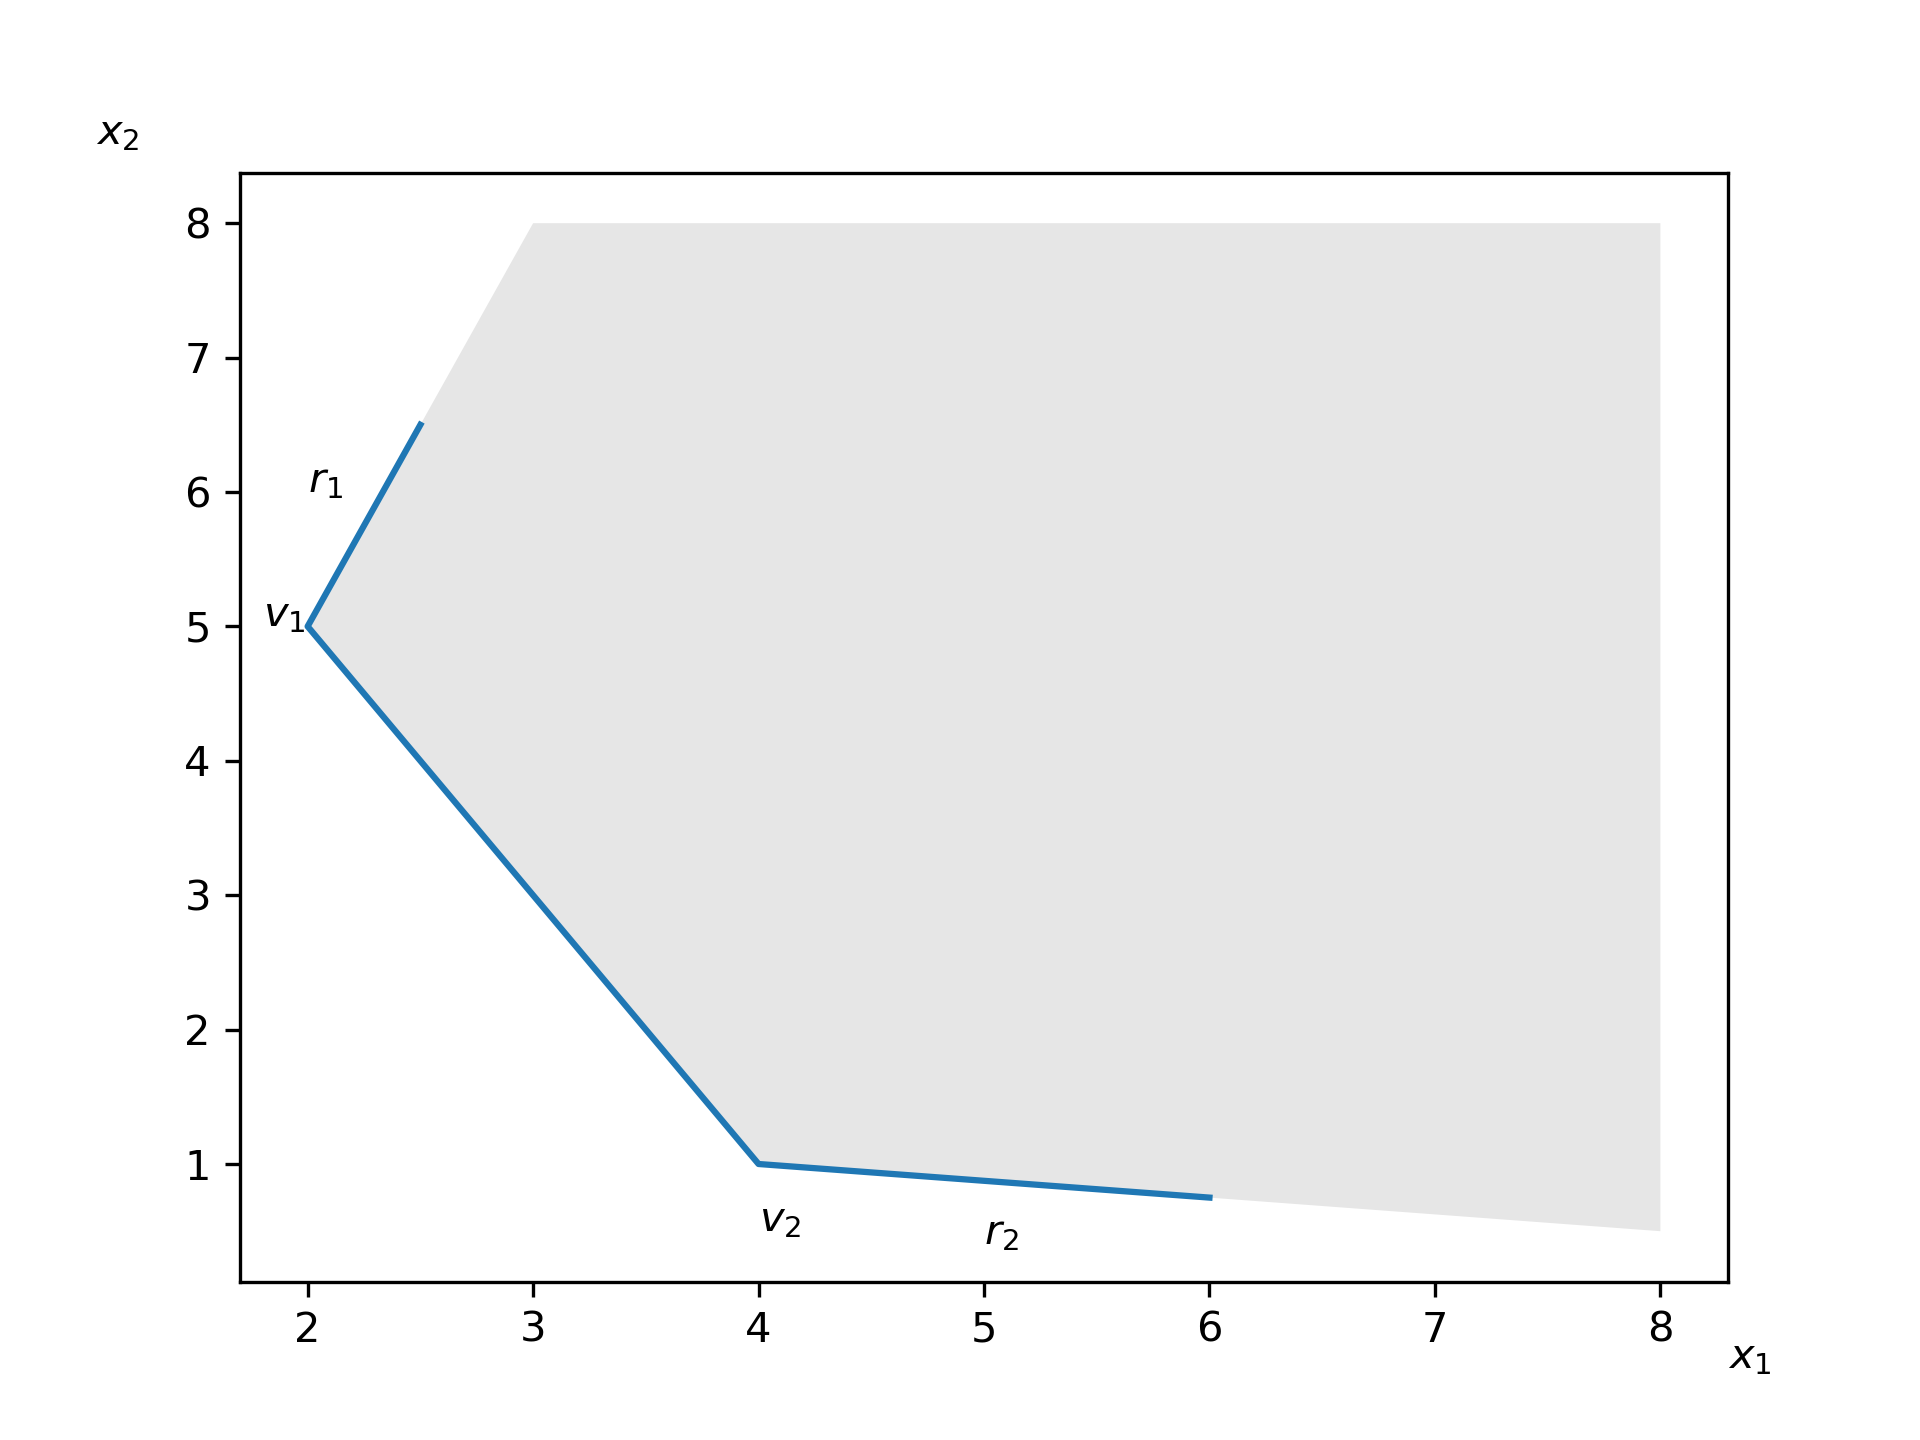
\includegraphics[scale = 0.7]{images/2022-09-27_lin_prog_1_03.png}
\end{figure}

With this machinery in place, the book (Theorem 2.1.2) defines the feasible region $\Fc$ of a linear program as combination of vertices $\vbf_1, \ldots, \vbf_k$ and extreme directions $\rbf_1, \ldots, \rbf_l$,

\bee
\xbf = \lambda_1 \vbf_1 + \cdots + \lambda_k \vbf_k + \mu_1 \rbf_1 + \cdots + \mu_l \rbf_l
\eee

with $\lambda_1 + \cdots + \lambda_k = 1$ and $\lambda_1, \ldots, \lambda_k, \mu_1, \ldots, \mu_l \geq 0$.

If the feasible region $\Fc$ is bounded (i.e. there are no vectors $\rbf$), then the feasible region is given by the convex hull of its vertices $\vbf_i$ (as the lambdas need to sum up to one). If it is unbounded, the feasible region consists of the convex hull of its vertices, shifted along a linear combination of directions of unboundedness.

In our example above, the feasible region is defined as

\bee
\xbf = \lambda \vbf_1 + (1-\lambda) \vbf_2 + \mu_1 \rbf_1 + \mu_2 \rbf_2, \quad \lambda, \mu_1, \mu_2 \geq 0
\eee

If we fix $\lambda = 1/2$ and define $\xbf_0 = \frac{1}{2} \vbf_1 + \frac{1}{2} \vbf_2$, then above equation (i.e. by varying $\mu_1$ and $\mu_2$) spans the dark region in the following Figure. By choosing different values of $\lambda$, the point $\xbf_0$ moves along the $\vbf_1 - \vbf_2$ line and the dark region wanders along.

\begin{figure}[H]
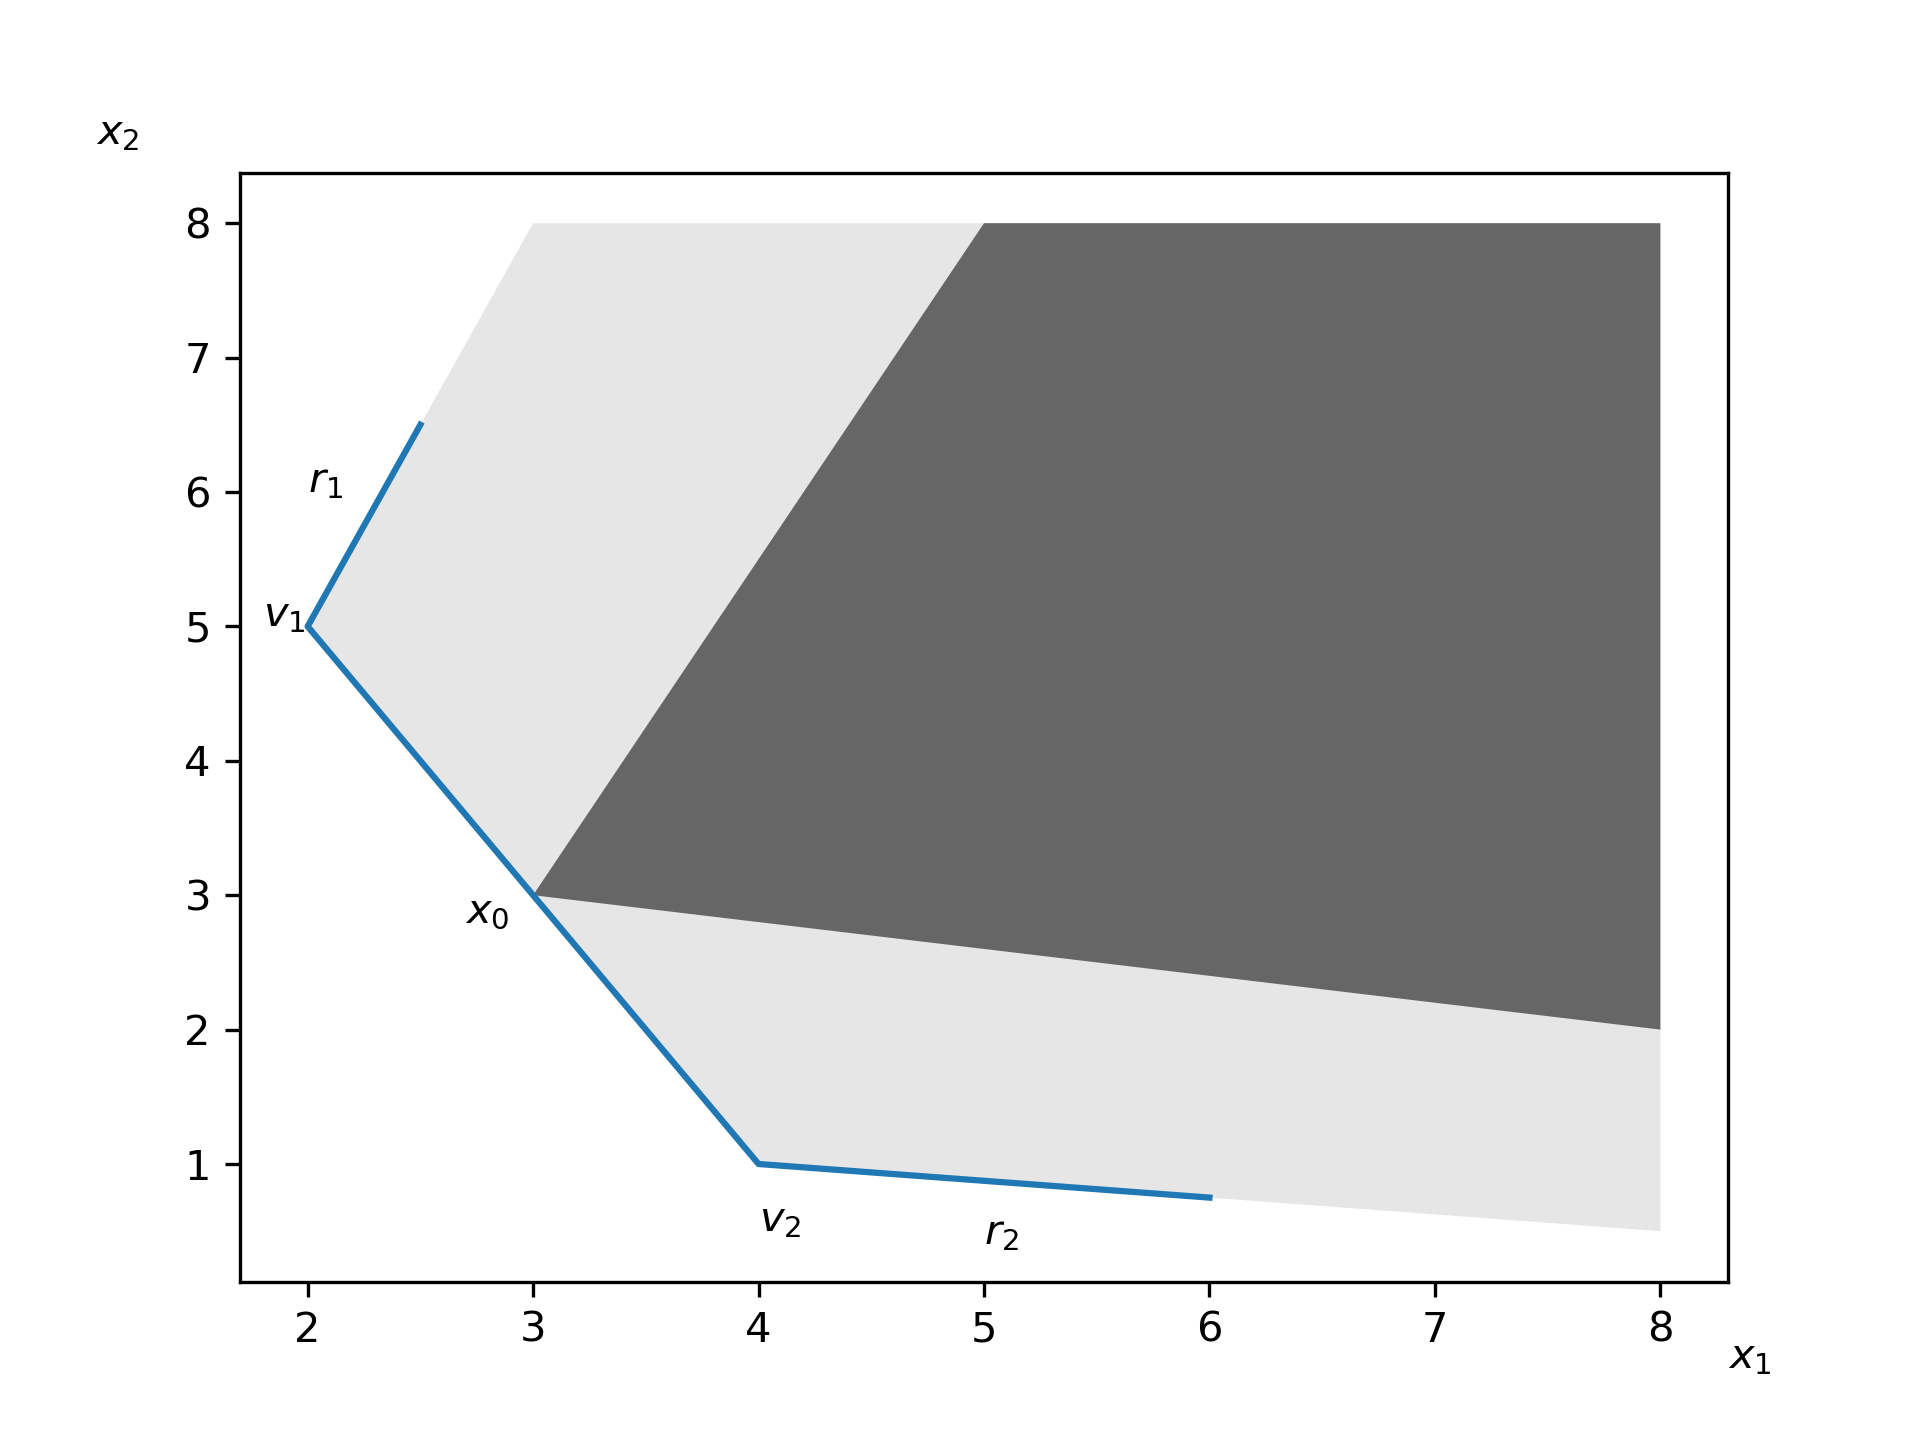
\includegraphics[scale = 0.7]{images/2022-09-27_lin_prog_1_04.png}
\end{figure}


\paragraph{Faces of the Feasible Region.} The constraints of the linear program in standard form are given by

\bee
\abf^T_j \xbf_j = b_j
\eee

for all $j = 1, \ldots, m+n$. Let us define a subset $J$ of $\{1,2,\ldots, m+n\}$ and its complement $\bar{J}$. Let $\Fc_J$ be the subset of the region $\Fc$ where all $\leq$ constraints with indices in $J$ are replaced by $=$ constraints,

\bee
\Fc_J = \{ \xbf \in \mR | \abf^T_j \xbf = b_j \forall  j \in J, \abf^T_i \xbf = b_i \forall  i \in \bar{J} \}
\eee

If $\Fc_J \neq 0$, then $\Fc_J$ is called a face of $\Fc$.

In our running example of the Dovetail model, the faces of the feasible region are vertces and lines. The lines are $\zerobf - \vbf_1, \vbf_1 - \vbf_2, \vbf_2 - \vbf_3, \vbf_3 - \vbf_4, \vbf_4 - \zerobf$. All these lines are given by $\Fc_J$ sets where $J$ has one element. Less intuitively, intersections are also faces; e.g. the vertex $\vbf_2$. This ``face'' is determined by the set

\bee
\{ \xbf \in \mR |3x_1 + x_2 = 18, x_1 + x_2 = 9, x_1 \leq 7, x_2 \leq 6, x_1 \geq 0, x_2 \geq 0 \}
\eee

which corresponds to a set $J$ with two elements.


\paragraph{Optimal Vertex Theorem.} This theorem states that if a linear program has an optimal solution, then the set of all optimal solutions is a face of the feasible region. We also have that the feasible region of any standard LO-model has at least one vertex. And finally, a standard linear program-model has an optimal solution if and only if its feasible region contains an optimal vertex.






\subsection{Simplex Algorithm}

The idea of the simplex algorithm is to manipulate the rows and columns of the technology matrix which corresponds to jumping from vertex to vertex of the feasible region $\Fc$. Since the optimal solution lies at a vertex of $\Fc$, we will eventually reach the optimum. A model with $n$ variables and $m$ constraints has up to ${m+n \choose m}$ vertices, which makes visting all of them infeasible The simplex algorithm considers the vertices in a more systematic way and is therefore more efficient. 

The simplex algorithm starts at a vertex of the feasible region and continues by choosing an adjacent vertex with larger objective value. The algorithm stops when the objective value cannot be improved by choosing a new adjacent vertex.

\todo{Explain the algorithm in more detail} 

We can use Julia to solve the Dovetail model; the source code is here (no big surprises). Optimum values are $x_1 = x_2 = 4.5$, yielding an optimum value of $22.5$. We have also calculated the slack and can see that we fully utilize the first two constraints, whereas there is some slack left in constraints three and four.

\begin{verbatim}
julia> println(objective_value(model))
22.5

julia> println("amounts = ", value.(m))
amounts = [4.5, 4.5]

julia> A*value.(m) - r
4-element Vector{Float64}:
  0.0
  0.0
 -2.5
 -1.5
\end{verbatim}

\subsection{Appendix: Convex Sets}

Consider an inequality

\bee
\Abf \xbf \leq \bbf
\eee

which describes a convex region; as an example consider a two-dimensional case with the following three inequalities,

\begin{align*}
  x_1 &\leq 3 \\
  x_2 &\leq 4 \\
  x_1 + x_2 &\leq 6
\end{align*}

We can collect this in a matrix-vector form as

\bee
\begin{pmatrix} 1 & 0 \\ 0 & 1 \\ 1 & 1 \end{pmatrix} \begin{pmatrix} x_1 \\ x_2 \end{pmatrix}  \leq \begin{pmatrix} 3 \\ 4 \\ 6 \end{pmatrix}
\eee

Now consider two points $\pbf_1, \pbf_2$ in the convex region; i.e. $\Abf \pbf_i \leq \bbf$. The points are connected by a line $\lambda \pbf_1 + (1-\lambda) \pbf_2$ with $\lambda \in [0,1]$. For $\lambda$ outside this interval, the points are "outside" the line connecting $\pbf_1$ and $\pbf_2$.

We want to show that all points between $\pbf_1$ and $\pbf_2$ are also in the convex region. We have

\bee
\Abf ( \lambda \pbf_1 + (1-\lambda) \pbf_2) = \lambda \Abf \pbf_1 + (1-\lambda) \Abf \pbf_2
\eee

The points are in the convex region; so $\Abf \pbf_i \leq \bbf$. If $\lambda \in [0,1]$ then $1-\lambda$ is positive as well (more exactely, it is $ \in [0,1]$) and \emph{only then} we are allowed to continue as

\bee
\lambda \Abf \pbf_1 + (1-\lambda) \Abf \pbf_2 \leq \lambda \bbf + (1-\lambda) \bbf = \bbf \qed
\eee



%%% Local Variables:
%%% mode: latex
%%% TeX-master: "journal"
%%% End:
